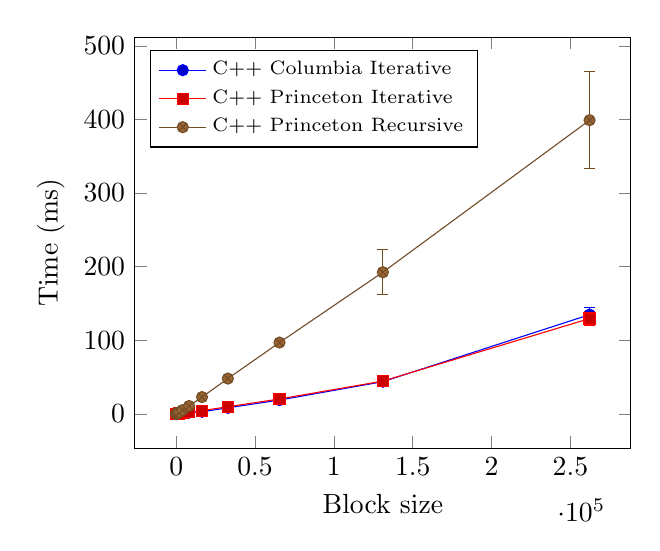
\begin{tikzpicture}
\begin{axis}[xlabel={Block size},ylabel={Time (ms)},width=0.65\linewidth,legend pos=north west,scaled y ticks = false,legend cell align=left,legend style={font=\scriptsize}]
\addplot+[error bars/.cd, y dir=both,y explicit] coordinates {
(16, 0.0049) +- (0.0015, 0.0015)
(32, 0.0051) +- (0.0002, 0.0002)
(64, 0.0052) +- (0.0005, 0.0005)
(128, 0.0071) +- (0.0003, 0.0003)
(256, 0.0160) +- (0.0408, 0.0408)
(512, 0.0223) +- (0.0032, 0.0032)
(1024, 0.0516) +- (0.0547, 0.0547)
(2048, 0.1206) +- (0.0787, 0.0787)
(4096, 0.8794) +- (0.4366, 0.4366)
(8192, 1.8030) +- (0.9841, 0.9841)
(16384, 2.9629) +- (0.6687, 0.6687)
(32768, 8.2847) +- (1.2061, 1.2061)
(65536, 18.8158) +- (2.8032, 2.8032)
(131072, 43.7807) +- (6.4454, 6.4454)
(262144, 134.8093) +- (10.2633, 10.2633)
};
\addplot+[error bars/.cd, y dir=both,y explicit] coordinates {
(16, 0.0090) +- (0.0022, 0.0022)
(32, 0.0128) +- (0.0052, 0.0052)
(64, 0.0188) +- (0.0029, 0.0029)
(128, 0.0292) +- (0.0032, 0.0032)
(256, 0.0541) +- (0.0048, 0.0048)
(512, 0.1038) +- (0.0056, 0.0056)
(1024, 0.2082) +- (0.0127, 0.0127)
(2048, 0.4536) +- (0.0536, 0.0536)
(4096, 0.9690) +- (0.0314, 0.0314)
(8192, 2.0605) +- (0.0561, 0.0561)
(16384, 4.5027) +- (0.1737, 0.1737)
(32768, 9.6797) +- (0.6568, 0.6568)
(65536, 20.3049) +- (1.7691, 1.7691)
(131072, 44.5770) +- (4.8859, 4.8859)
(262144, 129.5150) +- (9.2859, 9.2859)
};
\addplot+[error bars/.cd, y dir=both,y explicit] coordinates {
(16, 0.0215) +- (0.0225, 0.0225)
(32, 0.0328) +- (0.0031, 0.0031)
(64, 0.0617) +- (0.0047, 0.0047)
(128, 0.1252) +- (0.0086, 0.0086)
(256, 0.2642) +- (0.0405, 0.0405)
(512, 0.5573) +- (0.0791, 0.0791)
(1024, 1.1380) +- (0.0245, 0.0245)
(2048, 2.4265) +- (0.0476, 0.0476)
(4096, 5.1699) +- (0.2963, 0.2963)
(8192, 10.7496) +- (0.2605, 0.2605)
(16384, 22.8640) +- (0.8917, 0.8917)
(32768, 48.0022) +- (1.2536, 1.2536)
(65536, 96.9572) +- (1.3564, 1.3564)
(131072, 192.4607) +- (30.4597, 30.4597)
(262144, 398.9698) +- (65.9217, 65.9217)
};
\legend{C++ Columbia Iterative , C++ Princeton Iterative , C++ Princeton Recursive}
\end{axis}
\end{tikzpicture}
